\documentclass[../main.tex]{subfiles}
\begin{document}
Write a program that creates a user interface to perform integer divisions.
The user enters two numbers in the text fields, Num1 and Num2. The division of
Num1 and Num2 is displayed in the Result field when the Divide button is
clicked. If Num1 or Num2 were not an integer, the program would throw a
NumberFormatException. If Num2 were zero, the program would throw an Arithmetic
Exception Display the exception in a message dialog box.

\subsection{Code}
\inputminted[frame=lines, breaklines, breakanywhere, numberblanklines=false]{java}{./programs/prog16/Dialog.java}

\subsection{Output}
\begin{figure}[h!]
	\centering
	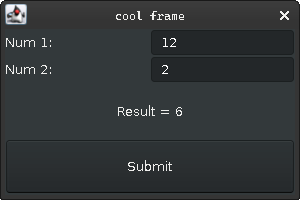
\includegraphics[width=0.4\textwidth]{./assets/p16-s1.png}
\end{figure}
\begin{figure}[h!]
	\centering
	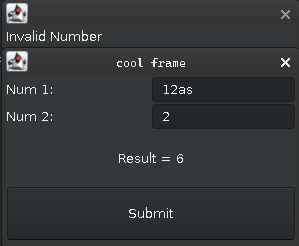
\includegraphics[width=0.4\textwidth]{./assets/p16-s2.png}
	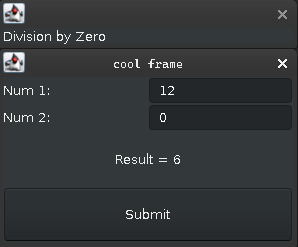
\includegraphics[width=0.4\textwidth]{./assets/p16-s3.png}
\end{figure}

\end{document}
